\documentclass{article}   

\usepackage{amssymb}
\usepackage{amsfonts}
\usepackage{hyperref}
\usepackage{eqnarray,amsmath}
\usepackage[table]{xcolor}
%
% \usepackage{mathptmx}      % use Times fonts if available on your TeX system
%
% insert here the call for the packages your document requires
%\usepackage{latexsym}
% etc.
%
\usepackage{graphicx}
\usepackage[round]{natbib}

\usepackage[table]{xcolor}
\usepackage{rotating}
\usepackage{caption}

%% if you use PostScript figures in your article
%% use the graphics package for simple commands
\usepackage{graphics}
\usepackage{natbib}


%% or use the graphicx package for more complicated commands
\usepackage{graphicx}
\usepackage[table]{xcolor}
% please place your own definitions here and don't use \def but
% \newcommand{}{}
%
% Insert the name of "your journal" with
% \journalname{myjournal}
%
\begin{document}

\title{Exercises of chapter 1}


\maketitle
Mayra Cristina Berrones Reyes

\section{Approximation}

Determine experimentally in which situations it is convenient to resort to approximations of the factorial like Equation \ref{eq1} and Equation \ref{eq2}. That is to say, how much computational time is saved, and at what precision cost. Additionally, what happens if the values ??of $e$ are also approximates. (For example, with Equation \ref{eq1} or \ref{eq2} or some other of the various forms that are known to approximate their value) and of $\pi$ (for which there are numerous approximations) instead of assuming they were constants of fixed precision.\\

Factorial numbers can be used in combinational probability, to calculate combinations and permutations. Through this, factorials are also often used to calculate probabilities, such as binomial coefficient  where ! marks the factorial number, and it is defined as all integer number k $\in \mathbb{Z}$, such as

\begin{eqnarray}
\label{eq3}
k! = k * (k - 1) * (k - 2) *... * 2 *1
\end{eqnarray}

A very useful approximation  of the factorial is the Stirling approximation:

\begin{eqnarray}
\label{eq1}
k! \approx k^{k} e^{-k} \sqrt{2\pi k}	
\end{eqnarray}

and the improved version by Gosper:

\begin{eqnarray}
\label{eq2}
k! \approx \sqrt{\pi (2k + \frac{1}{3})} k^{k} e^{-k}
\end{eqnarray}

This approximations are used when the factorial number is too big. However, this approximations come with various degrees of error. Equation \ref{eq4} shows the formula to get the percentage error.

\begin{eqnarray}
\label{eq4}
E = \mid \frac{Tv - Av}{Tv}	 \mid * 100\%
\end{eqnarray}

Where: \\

E: Percentage error.\\
Tv: True value\\
Av: Approximation value\\

In Python the library math has already a fixed parameter for the value $\pi$ and \textit{e}.

\begin{figure}[htp]
	\centering
	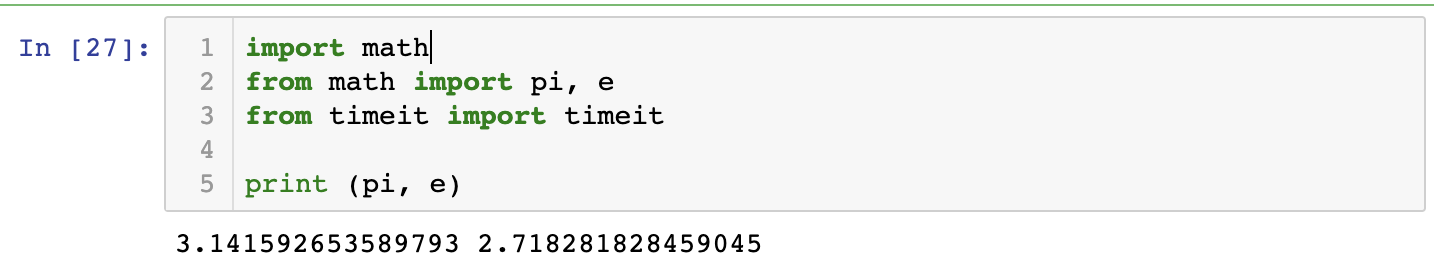
\includegraphics[width=\linewidth]{math.png}
	\label{meatj}
\end{figure}

First we begin our experiment by taking those parameters of $\pi$ and \textit{e} from the math library, and using the Stirling approximation. \footnote{All experimentation mentioned we used a code in python, and it can be consulted here: } In Table \ref{ta1} we can se the results. Column N is the number we used to take the value of the factorial. N! is the answer provided by python form the same math library, and the column Stirling is the approximation. Time is the processing time it took to compile, and the error was calculated with Equation \ref{eq4}.

\begin{table}[h!]
\centering
 \caption{Results of the Stirling approximation} 
 \label{ta1}
 \begin{tabular} {| l | l | l | l | l |}
 \hline
\textbf{N}	&	\textbf{N!}	&	\textbf{Stirling} 	&	\textbf{Time}	&	\textbf{Error}	\\
\hline
1	&	1	&	0.922137009	&		&	0.077862991	\\
\hline
5	&	120	&	118.941305	&	0.000825167	&	0.008822459	\\
\hline
10	&	3628800	&	3598814.56	&	0.001646757	&	0.008263183	\\
\hline
25	&	1.55112E+25	&	1.54596E+25	&	0.001966	&	0.003327607	\\
\hline
50	&	3.04141E+64	&	3.03634E+64	&	0.002142906	&	0.001665256	\\
\hline
75	&	2.4809E+109	&	2.4782E+109	&	0.002707958	&	0.001110487	\\
\hline
100	&	9.3326E+157	&	9.3248E+157	&	0.002886772	&	0.000832983	\\
\hline
125	&	1.8827E+209	&	1.8814E+209	&	0.003069878	&	0.000666443	\\
\hline
130	&	6.4669E+219	&	6.4627E+219	&	0.003262997	&	0.000640819	\\
\hline
 \end{tabular}
 \end{table}
 
 Then in Table \ref{ta2} we have the results of the Gosper Equation \ref{eq2}.
 
 \begin{table}[h!]
\centering
 \caption{Results of the Gosper approximation.} 
 \label{ta2}
 \begin{tabular} {| l | l | l | l | l |}
 \hline
\textbf{N}	&	\textbf{N!}	&	\textbf{Gosper} 	&	\textbf{Time}	&	\textbf{Error}	\\
\hline
1	&	1	&	0.996021807	&		&	0.003978193	\\
\hline
5	&	120	&	120.966052	&	0.012824059	&	-0.008050433	\\
\hline
10	&	3628800	&	3628681.791	&	0.013508797	&	3.25753E-05	\\
\hline
25	&	1.55112E+25	&	1.5511E+25	&	0.013875008	&	1.08842E-05	\\
\hline
50	&	3.04141E+64	&	3.0414E+64	&	0.014073133	&	2.7494E-06	\\
\hline
75	&	2.4809E+109	&	2.4809E+109	&	0.014258862	&	1.22616E-06	\\
\hline
100	&	9.3326E+157	&	9.3326E+157	&	0.016538858	&	6.90896E-07	\\
\hline
125	&	1.8827E+209	&	1.8827E+209	&	0.016858816	&	4.42627E-07	\\
\hline
130	&	6.4669E+219	&	6.4669E+219	&	0.017882824	&	4.09269E-07	\\
\hline
 \end{tabular}
 \end{table}
 
 We see that the bigger the value of N, the approximation gets similar to the true value.\\
 
 As the next step on our experimentation, we wanted to explore a little more inside the formulas of Stirling and Gosper, since both of them use the $\pi$ and \textit{e} values, and they are approximations as well.\\
 
Both of this values have formulas to get a better approximation to its real value. For example, Equation \ref{eq6} for the $\pi$ value called the Leibniz formula, and Equation \ref{eq7} for the \textit{e} value. In Table \ref{ta3} the column of Value for $\pi$ and e is the value of n in the equations.\\

\begin{eqnarray}
\label{eq6}
\pi = 4 * \sum_{n=0}^{\infty} \frac{(-1)^n}{2n+2} = \frac{\pi}{4}
\end{eqnarray}

\begin{eqnarray}
\label{eq7}
e = (1 + \frac{1}{n})^n
\end{eqnarray}
 
  \begin{table}[h!]
\centering
 \caption{Description of the distribution of the values for $\pi$ and \textit{e}.} 
 \label{ta3}
 \begin{tabular} {| l | l | l | }
 \hline
\textbf{Value for $\pi$ and e}	&	\textbf{$\pi$}	&	\textbf{e} \\
\hline				
10	&	3.041839619	&	2.59374246\\
\hline
100	&	3.131592904	&	2.704813829\\
\hline
1000	&	3.140592654	&	2.716923932\\
\hline
10000	&	3.141492654	&	2.718145927\\
\hline
100000	&	3.141582654	&	2.718268237\\
\hline
1000000	&	3.141591654	&	2.718280469\\
\hline
10000000	&	3.141592554	&	2.718281694\\ 
\hline
100000000	&	3.141592644	&	2.718281798\\

\hline
 \end{tabular}
 \end{table}
 
 Now we show the results of the experimentation in Table \ref{ta4} and \ref{ta5}. Here is where the computational time shows some significance, because in the larger ones, it took more than a minute to compile and give us an answer.\\
 
 
   \begin{table}[h!]
\centering
 \caption{Results of the Stirling approximation using the different values of $\pi$ and e} 
 \label{ta4}
 \begin{tabular} {| l | l | l | l | l | }
 \hline
\textbf{N}	&	\textbf{N!}	&	\textbf{Stirling}	&	\textbf{Time}	&	\textbf{Error}	\\
\hline
1	&	1	&	0.922232625	&		&	0.077767375	\\
\hline
5	&	120	&	147.7417932	&	0.002756834	&	-0.23118161	\\
\hline
10	&	3628800	&	3776077.14	&	0.004431009	&	-0.040585632	\\
\hline
25	&	1.55112E+25	&	1.56514E+25	&	0.009263992	&	-0.009039953	\\
\hline
50	&	3.04141E+64	&	3.0439E+64	&	0.04496026	&	-0.000817607	\\
\hline
75	&	2.4809E+109	&	2.4791E+109	&	0.343361855	&	0.000737427	\\
\hline
100	&	9.3326E+157	&	9.3253E+157	&	2.778558016	&	0.000783175	\\
\hline
125	&	1.8827E+209	&	1.8814E+209	&	25.75114012	&	0.000660286	\\
\hline
130	&	6.4669E+219	&	6.4627E+219	&	251.0401418	&	0.000639381	\\
\hline
 \end{tabular}
 \end{table}
 
 
\begin{table}[h!]
\centering
 \caption{Results of the Gosper approximation using the different values of $\pi$ and e.} 
 \label{ta5}
 \begin{tabular} {| l | l | l | l | l | }
 \hline
\textbf{N}	&	\textbf{N!}	&	\textbf{Gosper}	&	\textbf{Time}	&	\textbf{Error}	\\
\hline
1	&	1	&	1.527525232	&	0	&	-0.527525232	\\
\hline
5	&	120	&	150.7740198	&	0.00718689	&	-0.256450165	\\
\hline
10	&	3628800	&	3807416.223	&	0.005645037	&	-0.049221843	\\
\hline
25	&	1.55112E+25	&	1.57035E+25	&	0.012120962	&	-0.012397832	\\
\hline
50	&	3.04141E+64	&	3.04896E+64	&	0.056209087	&	-0.002484249	\\
\hline
75	&	2.4809E+109	&	2.4818E+109	&	0.380222797	&	-0.000372249	\\
\hline
100	&	9.3326E+157	&	9.3331E+157	&	3.328314781	&	-4.91594E-05	\\
\hline
125	&	1.8827E+209	&	1.8827E+209	&	30.81744933	&	-5.71849E-06	\\
\hline
130	&	6.4669E+219	&	6.4669E+219	&	299.2242897	&	-1.02921E-06	\\
\hline
 \end{tabular}
 \end{table}
 
 \section{Conclusions} 
 
 At the end of the experimentation, we noticed that the second part of the experiment, when we began to change the parameters of $\pi$ and e, the computational time started to grow, and comparing the first results where we used the default ones given by python, there is not much difference in accuracy of the approximation on the bigger numbers.\\
 
 On the smaller numbers, the difference between the first and the second experiment is quite noticeable. This being because the accuracy of the $\pi$ and e values are not very good.\\
 
With this we conclude that the accuracy of the $\pi$ and e values are very significant on the result of the Stirling and Gosper approximation formulas. Also, the Gosper formula proves to be the more accurate of the two on the bigger numbers.\\
 
\end{document}